% report-template.tex — the shape of a BNJetTag note. Copy, rename, fill. Compile: tectonic -X compile <file>.tex
\documentclass[11pt]{article}
\usepackage{bnjettag}
\title{\Large Title stating the result, not the topic}
\author{Kai Yamaguchi, UC San Diego}
\date{2026-09-26}
\begin{document}
\maketitle
\section*{Question}
One paragraph: the question, its null, and what would have falsified the claim.
\section*{Design}
Arms, seeds, selection rule (pre-registered), budget. Reference \texttt{STUDY.md}.
\section*{Result}
Numbers from \texttt{VERIFY.md} only, each labelled: \testauc{0.9xx}\singleseed. \\
\provenance{local/<study>/VERIFY.md}
\begin{figure}[h]\centering
  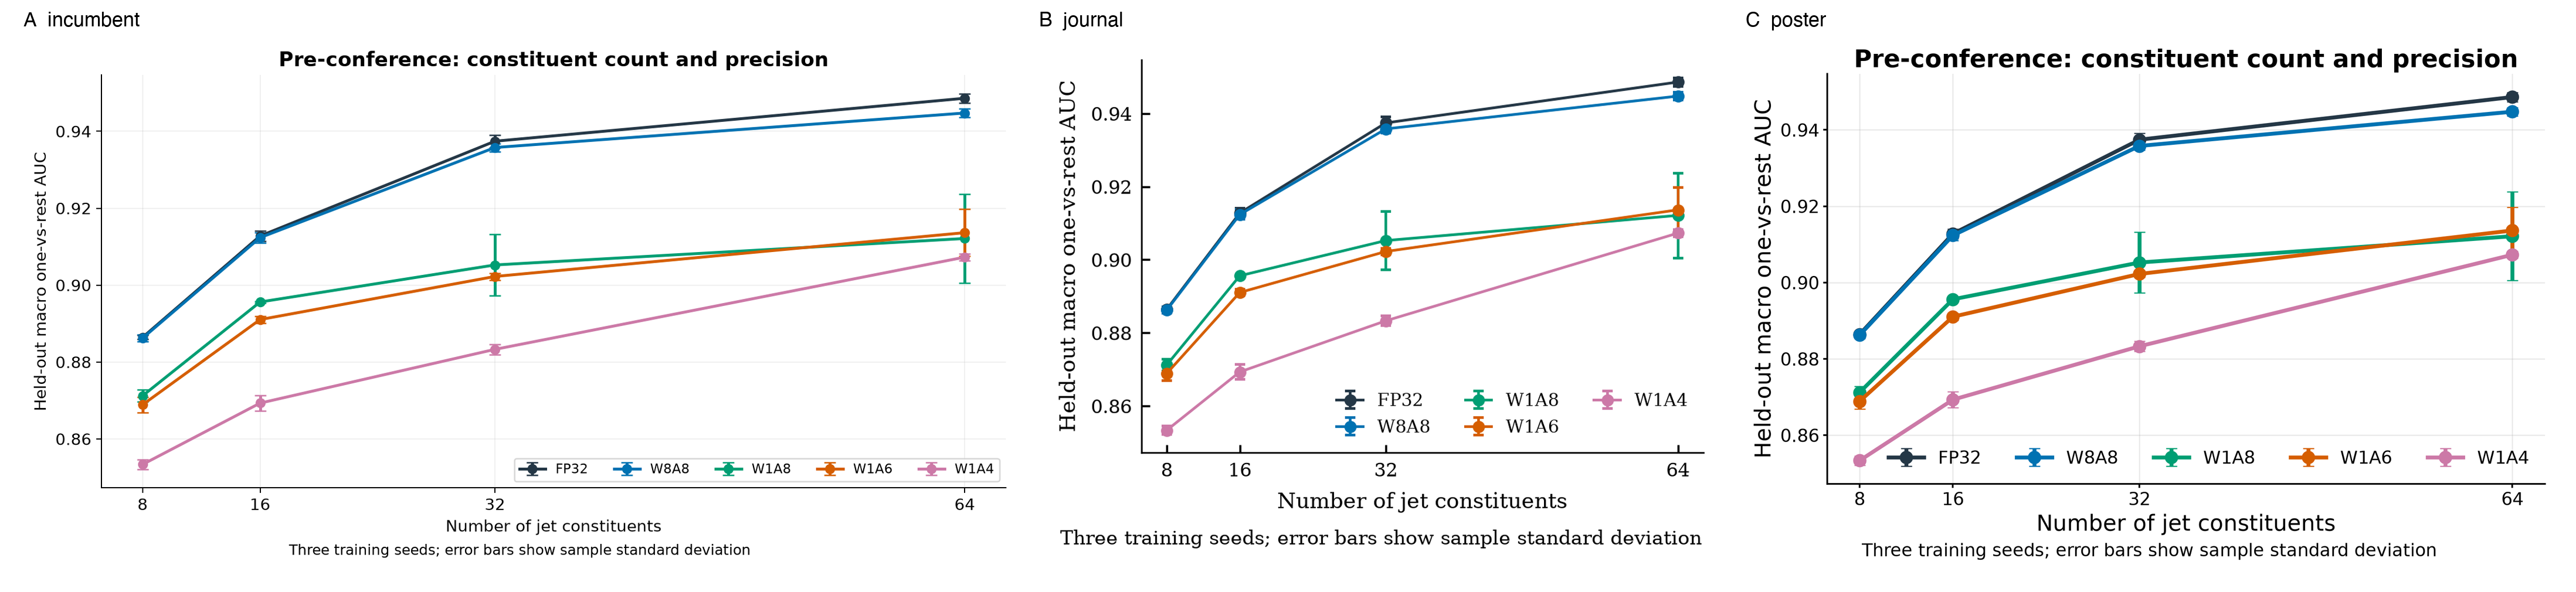
\includegraphics[width=\linewidth]{../figures/style/contact-sheet-auc.png}
  \caption{Three-seed held-out macro one-vs-rest AUC against constituent count, under three candidate styles (the journal style, centre, is the pick). Error bars: sample standard deviation over seeds.}
\end{figure}
\section*{Interpretation}
What this says about the thesis. What is still open.
\end{document}
